\documentclass[12pt]{article}
\usepackage[english]{babel}
\usepackage[utf8x]{inputenc}
\usepackage{amsmath}
\usepackage{graphicx}
\usepackage{parskip}
\usepackage{ucs}
\usepackage{float}
\usepackage{array}
\usepackage{amsmath}
\usepackage{amssymb}
\usepackage{amsfonts}
\usepackage{latexsym}
\usepackage{graphicx}
\usepackage{caption}
\usepackage{ifpdf}
\usepackage{url}
\usepackage{xtab}
\usepackage{geometry}
\usepackage{longtable}
\usepackage{tabularx}
\usepackage{booktabs}
\usepackage[hidelinks]{hyperref}

\newcommand{\HRule}{\rule{\linewidth}{1mm}}
\parskip 7.0pt
\renewcommand{\baselinestretch}{1.5}
\begin{document}
\begin{titlepage}
\vspace*{\stretch{1}}
\noindent\HRule
\begin{center}
\huge
\noindent TDT4175 Information Systems \\ [7mm]
\large
\noindent\emph{\textbf{Group 19}}\\
\paragraph*{}
Bertrand Nils Mathieu Duquesnoy\\ 
Knut Aron Fludal\\
Michal Gačko\\ 
Lars Henrik Søreide Grytten\\
Agata Anna Jedryszek\\
Håvard Holmboe Lian \\
\end{center}
\noindent\HRule
\vspace*{\stretch{2}}
\end{titlepage}
\newpage
\pagenumbering{Roman} 
\tableofcontents
\newpage
\pagenumbering{arabic} 
\setcounter{page}{1}

%Input sections here
\chapter{Introduction}

Information is one of the most valuable resources of an organization. The NTNU’s information system is a computer-based information system, it is composed of several actors (figure \ref{fig:infsyscom})  that, put together, fill the role of an effective information system. However, the information doesn’t seem to be always easily accessible with the current NTNU’s information system.

The information system in the university is set up to help and to provide students with every kind of information they need. That is why the information must be accessible, accurate and complete. But, having good information is not enough, the system must be efficient, effective and have good performance standards to display properly and constantly the right information.

So, in order to avoid being misled by wrong information, the current system needs to be improved. The present report highlights some current problems and the solutions that can be brought.

\begin{figure}[H]
	\begin{center}
		\centerline{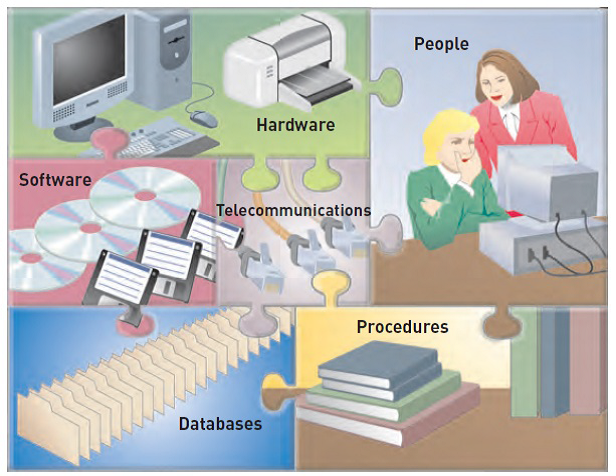
\includegraphics[scale=0.50]{infsyscom}}
		\caption[Computer-based information system components]{Computer-based information system components}
		\label{fig:infsyscom}
	\end{center}
\end{figure}



\end{document}